\documentclass[a4paper,12pt,fleqn]{article}%fleqn pour aligner les equations à gauche
\usepackage{Exercice}
\title{\vspace{-1cm}\large 
	\begin{tabular}{|>{\centering}m{5cm}|>{\centering}m{8cm}|>{\centering\arraybackslash}m{4cm}|}
		\hline
		Exercices & \textbf{\textsc{Lunette astronomique}} &  Chapitre 11 \\
		\hline
\end{tabular}
\vspace{-5em}}
\date{}

\begin{document}
	\maketitle
	
\begin{multicols}{2}
\section{Schématiser une lunette afocale}
\begin{center}
    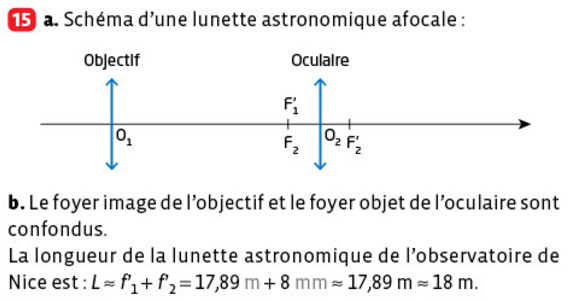
\includegraphics[width=\linewidth]{Ressources/TSPE_C11_Ex1.png}
\end{center}

\section{Définir un grossissement}
\begin{center}
    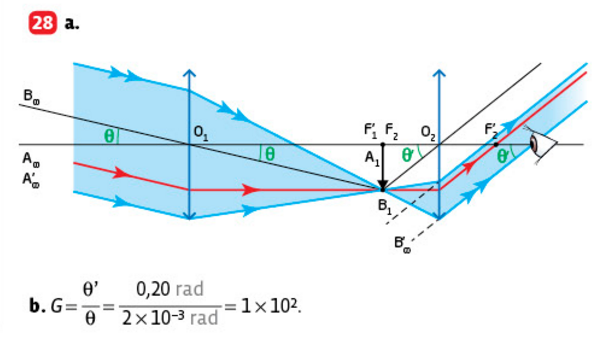
\includegraphics[width=\linewidth]{Ressources/TSPE_C11_Ex3.png}
\end{center}

\section{Pouvoir séparateur de l'\oe il}
\begin{center}
    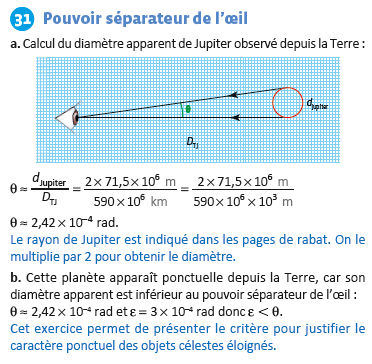
\includegraphics[width=\linewidth]{Ressources/TSPE_C11_Ex4.png}
\end{center}
\section{Étoiles doubles}
\begin{center}
    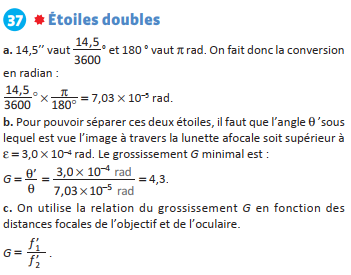
\includegraphics[width=\linewidth]{Ressources/TSPE_C11_Ex5-1.png}
    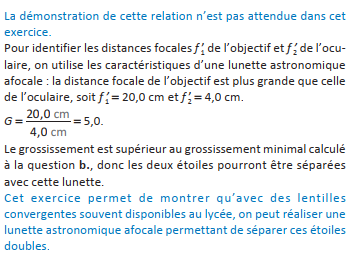
\includegraphics[width=\linewidth]{Ressources/TSPE_C11_Ex5-2.png}
\end{center}
\section{Drapeaux américains}
\begin{center}
    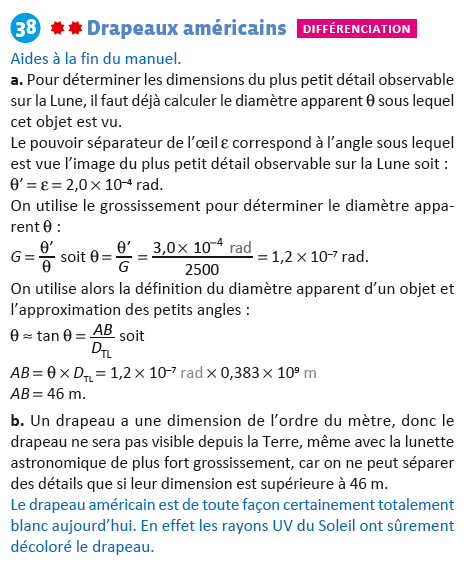
\includegraphics[width=\linewidth]{Ressources/TSPE_C11_Ex6.png}
\end{center}
\end{multicols}
\end{document}